% El piano
% Curso LaTeX y Git por Darwin Eventur
% Víctor Manuel Fernández Castro
% 16 de Enero de 2016

\documentclass[10pt,a4paper]{article}

\usepackage[utf8]{inputenc}
\usepackage[spanish]{babel}
\usepackage{lettrine}
\usepackage{graphicx}
\usepackage[skip=6pt]{caption}
\usepackage[hidelinks]{hyperref}

\title{El piano}
\author{Víctor Manuel Fernández Castro}

\setlength{\parskip}{6pt}

% ------------------------------------------------------------------------------

\begin{document}
	\maketitle
	\thispagestyle{empty}
	
	\begin{figure}[b]
		\centering
		
\includegraphics[width=2cm]{images/by-sa}
		\caption*{\textbf{Reconocimiento - CompartirIgual (by-sa)}: Se permite 
		el uso comercial de la obra y de las posibles obras derivadas, la 
		distribución de las cuales se debe hacer con una licencia igual a la 
		que regula la obra original.}
	\end{figure}
	
	\newpage
	\tableofcontents
	\listoffigures
	
	% Capítulo 1 ---------------------------------------------------------------
	
	\newpage
	\section{Origen e historia}
	
	\lettrine{E}{l piano} es un instrumento musical de cuerda percutida. El 
	término deriva de su nombre original en italiano: \textit{pianoforte}, que  
	significa \textit{''suave-fuerte''}. La razón para bautizarlo de esta 
	manera es que fue el primer instrumento de su género capaz de producir 
	sonidos con distintos matices de intensidad.
	
	\begin{figure}[!ht]
		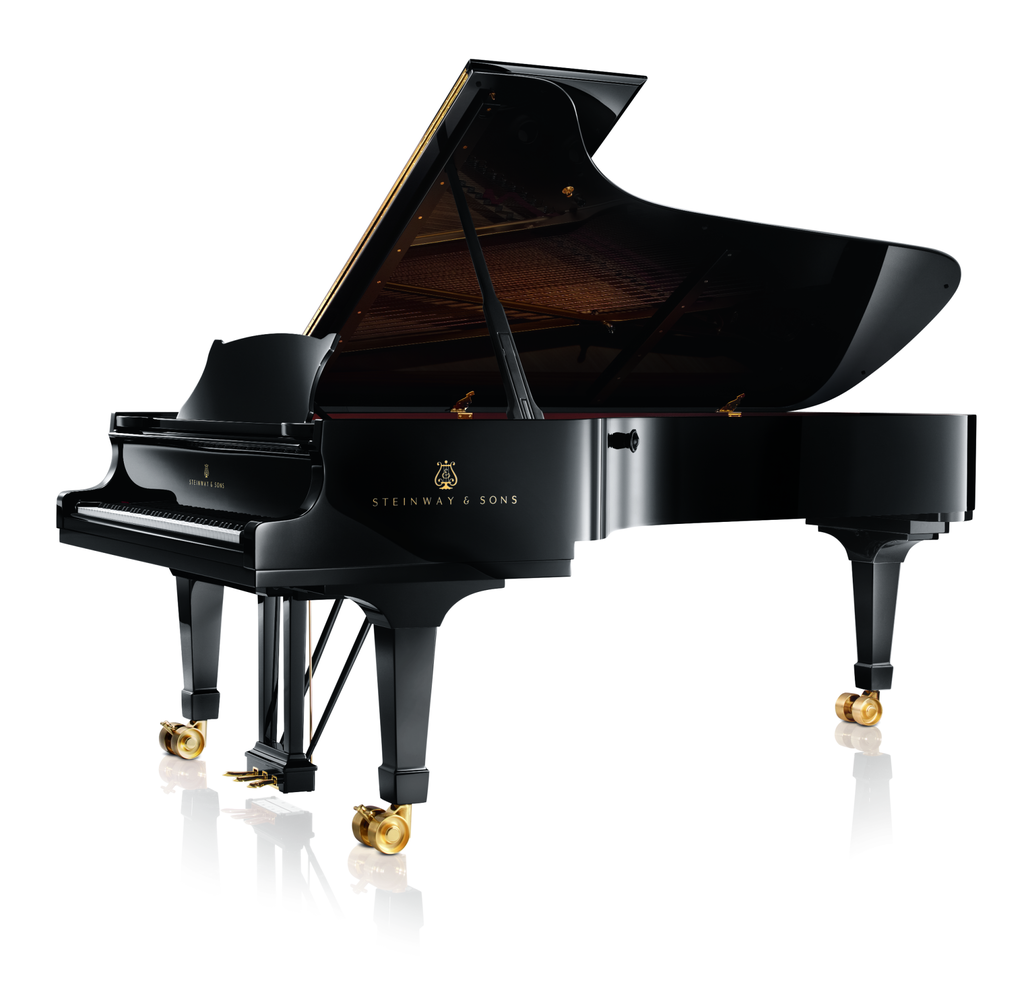
\includegraphics[width=\textwidth]{images/piano}
		\caption[Piano de cola]{\label{fig:piano} Piano de cola Steinway \& Sons. \cite{steinway}}
	\end{figure}
	
	Está formado por un teclado dotado de un mecanismo que transfiere las 
	pulsaciones del pianista a unos macillos forrados de fieltro que percuten 
	las cuerdas de acero que se hallan dentro de la caja de resonancia, y 
	transmiten las vibracionesa la tabla armónica, donde se amplifican.
	
	Su invención se remonta al año 1700 aproximadamente, y se atribuye a \textbf
	{Bartolomeo Cristofori}, un fabricante de clavicémbalos que fue  contratado 
	por el príncipe Fernando II de Medici como conservador de  instrumentos. 
	Cristofori construyó cerca de una veintena de pianos, hoy en día solo se 
	conservan tres.
	
	% Capítulo 2 ---------------------------------------------------------------
	
	\clearpage
	\section{Estructura}
	
	\subsection{Mecanismo de percusión}
	
	Cuando el pianista pulsa una tecla, la parte puesta se eleva y acciona un 
	juego de palancas que hace al apagador librar la cuerda y pone en 
	movimiento al macillo en dirección a la cuerda. Hacia la mitad del 
	recorrido, la palanca de escape se retira del rodillo y deja al macillo 
	libre, para golpear la cuerda por inercia. Al rebotar, la grapa atrapa al 
	macillo para evitar que vuelva a tocar la cuerda.
	
	Al soltar la tecla, el apagador presiona y silencia la cuerda, y el macillo 
	vuelve a su posición inicial. Todo este mecanismo hace que el macillo 
	toque la cuerda y vuelva inmediatamente para dejarla vibrar, y además 
	permite repetir rápidamente la misma nota.
	
	\begin{figure}[!ht]
		\centering
		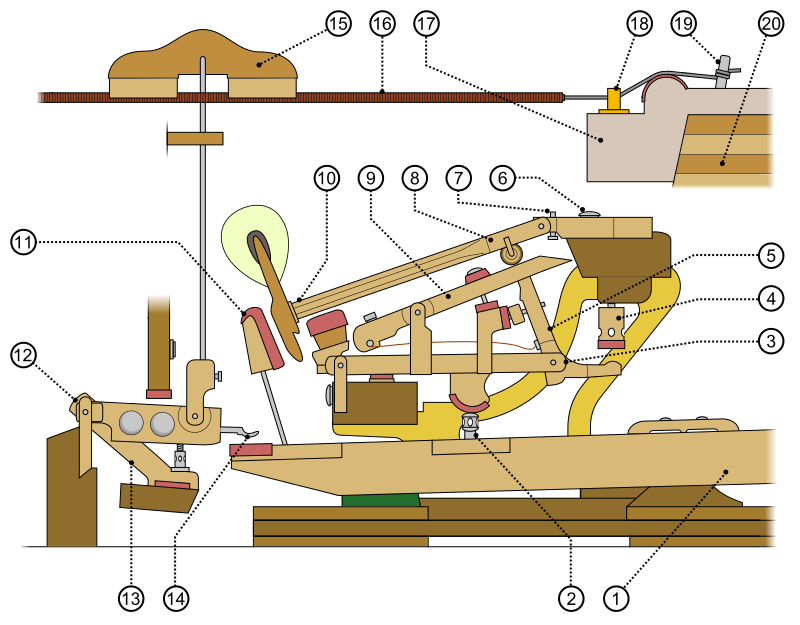
\includegraphics[width=0.75\textwidth]{images/pulsation}
		\caption[Mecanismo de pulsación]{\label{fig:pulsation} Mecanismo de pulsación en un piano de cola. \cite{pulsation}}
	\end{figure}
	
	\begin{table}[!ht]
		\centering
		\begin{tabular}{|r|l||r|l|}
			\hline
			1 & Tecla. & 11 & Atrape. \\
			2 & Pilotín. & 12 & Palanca del apagador. \\
			3 & Puente. & 13 & Palanca del pedal fuerte. \\
			4 & Pilotín de escape. & 14 & Cuchara del apagador. \\
			5 & Palanca de escape. & 15 & Apagador. \\
			6 & Tornillo de reborde del macillo. & 16 & Cuerda. \\
			7 & Rodillo. & 17 & Marco. \\
			8 & Brazo del macillo. & 18 & Grapa. \\
			9 & Palanca de repetición. & 19 & Clavija. \\
			10 & Cabeza del macillo. & 20 & Somier. \\
			\hline
		\end{tabular}
		\caption[Leyenda del mecanismo]{\label{tab:pulsation} Leyenda de la figura \ref{fig:pulsation}.}
	\end{table}
	
	\subsection{Caja de resonancia}
	
	La caja de resonancia es el recinto cerrado del piano y sirve para \textbf
	{amplificar} y modular el sonido. Es un factor decisivo en el \textbf
	{timbre} del instrumento.
	
	La \textbf{tabla armónica} es una superficie de madera laminada, se sitúa 
	debajo de los puentes y de las cuerdas. El \textbf{bastidor} es un armazón 
	de barras, generalmente de hierro, que soportan la tensión de todas las 
	cuerdas.
	
	\begin{figure}[!ht]
		\centering
		\includegraphics[width=0.5\textwidth]{images/interior}
		\caption[Caja de resonancia]{\label{fig:interior} Caja de resonancia de un piano de cola. \cite{interior}}
	\end{figure}
	
	\subsection{Cuerdas}
	
	Las cuerdas son los elementos vibratorios que originan el sonido. Los 
	bordones son las cuerdas de mayor longitud, están fabricadas en acero y 
	entorchadas con hilos de cobre. Pertenecen al registro grave del 
	instrumento y hay una sola cuerda por tecla, mientras que en el registro 
	medio se colocan dos cuerdas por tecla, y en el registro agudo, tres, cada 
	vez de menor longitud.
	
	\begin{figure}[!ht]
		\centering
		\includegraphics[width=0.5\textwidth]{images/strings}
		\caption[Cuerdas en un piano]{\label{fig:strings} Cuerdas en un piano de cola. \cite{strings}}
	\end{figure}
	
	La tensión de todas las cuerdas puede alcanzar de 15 a 20 toneladas. La 
	fabricación de una cuerda para piano se realiza mediante un proceso 
	denominado \textbf{trefilado}.
	
	\subsection{Teclado}
	
	La gran mayoría de pianos actuales tienen 88 teclas: 52 blancas y 36 
	negras, que corresponden a siete octavas y una tercera menor, desde 
	$La_{-1}$ hasta $Do_7$.
	
	\begin{figure}[!ht]
		\centering
		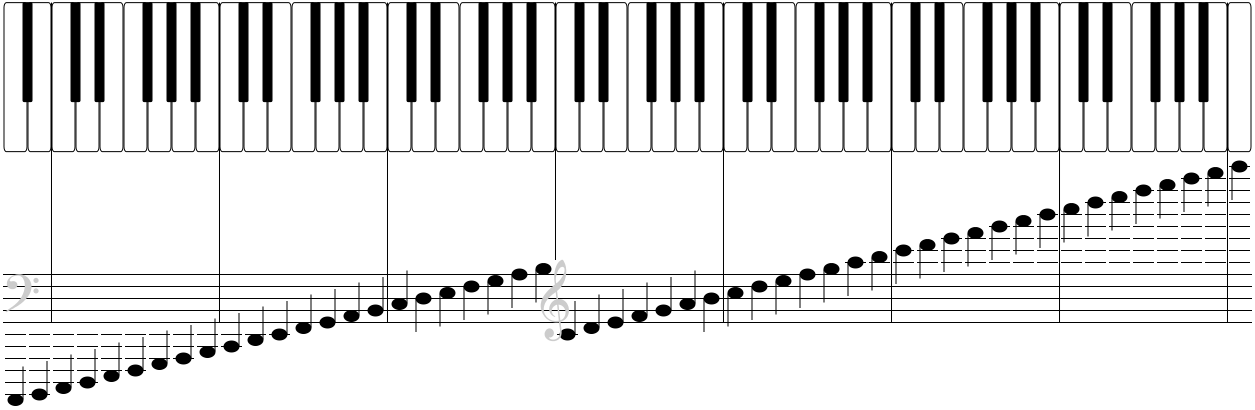
\includegraphics[width=\textwidth]{images/range}
		\caption[Extensión sonora]{\label{fig:range} Extensión sonora de un piano moderno. \cite{range}}
	\end{figure}
	
	\subsection{Pedales}
	
	Un piano moderno tiene hasta tres pedales, aunque a lo largo de la historia 
	ha cambiado su número y su función. Beethoven poseyó un piano con cinco 
	pedales ---dos de ellos complementarios---.
	
	\begin{description}
		\item[Pedal fuerte] Es el pedal derecho del piano. Al pisarlo, libera 
		los apagadores de las cuerdas, lo que permite que las notas sigan 
		sonando aun cuando se ha dejado de pulsar la tecla.
		
		\item[Pedal tonal] Se encuentra en el centro, crea un efecto parecido 
		al pedal fuerte, excepto que solo afecta a las notas que estén pulsadas 
		en el momento de pisarlo.
		
		\item[Pedal celeste] Situado a la izquierda, desplaza los macillos a un 
		lado para golpear menos cuerdas y, allá donde solo haya una, lo harán 
		de refilón, para dar un sonido más suave.
	\end{description}
	
	\begin{figure}[!ht]
		\centering
		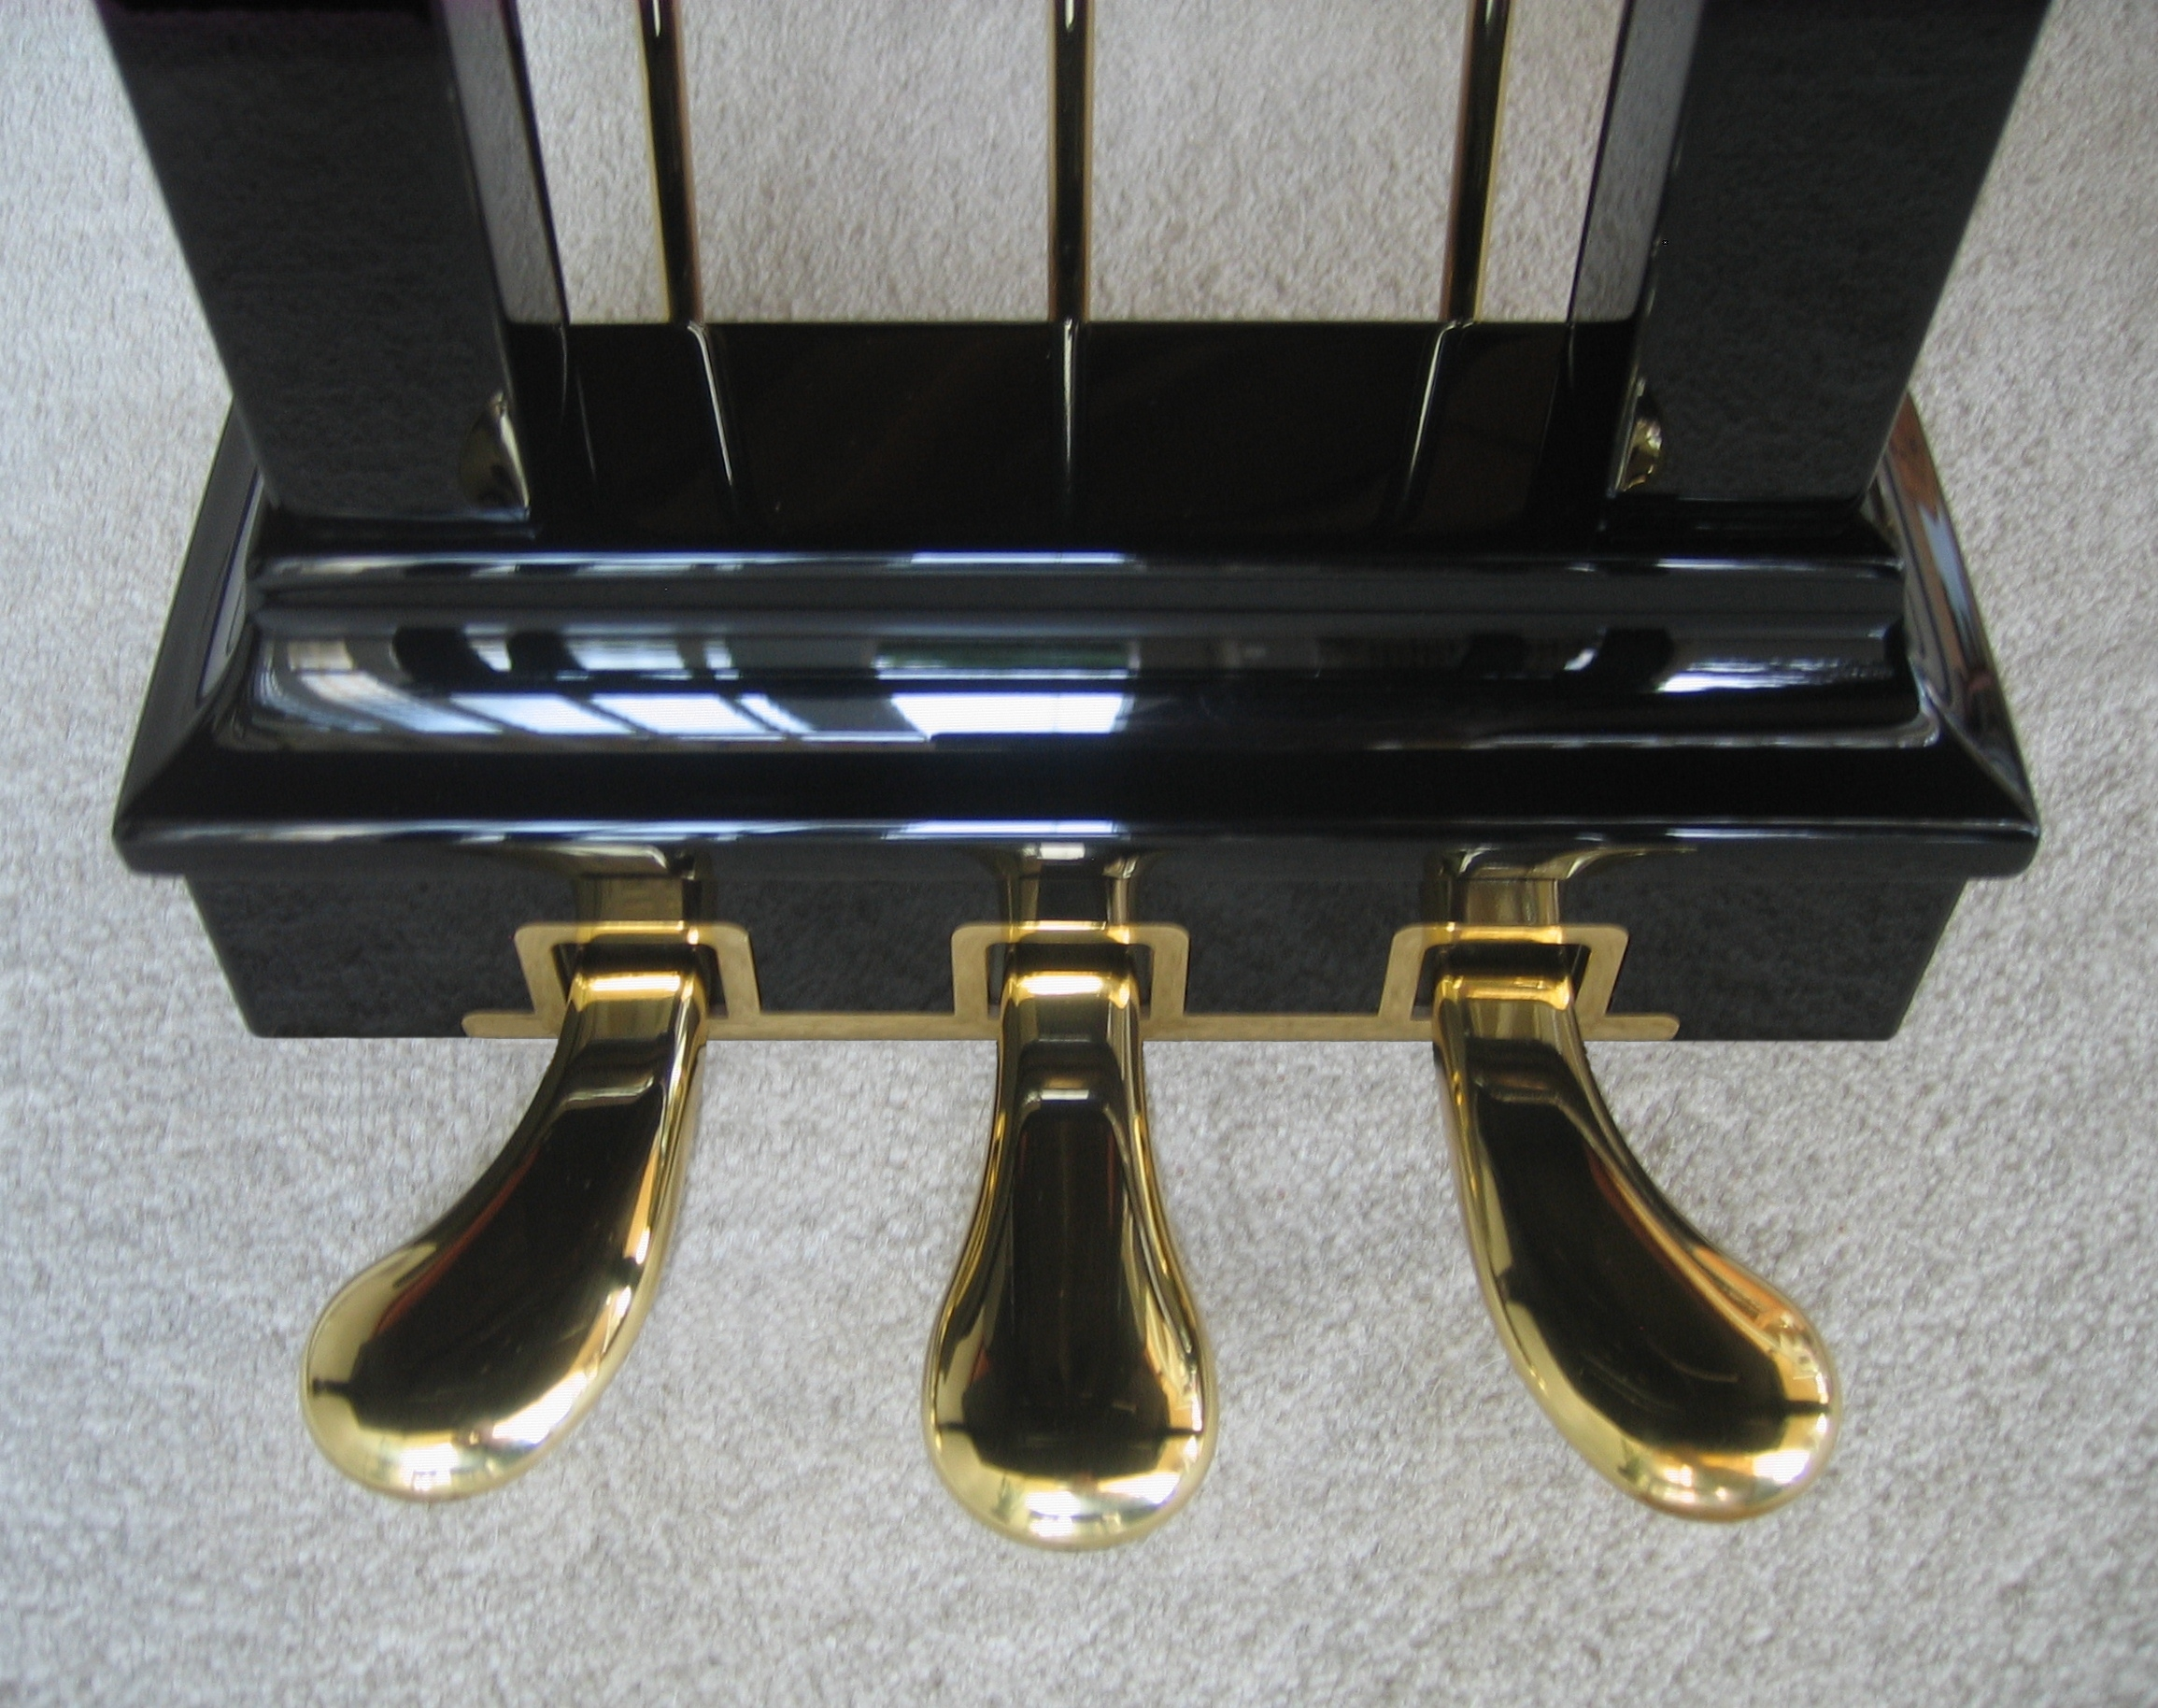
\includegraphics[width=0.5\textwidth]{images/pedals}
		\caption[Pedales de un piano]{\label{fig:pedals} Pedales de un piano. \cite{pedals}}
	\end{figure}
	
	% Capítulo 3 ---------------------------------------------------------------
	
	\clearpage
	\section{Afinación}
	
	Afinar un piano consiste en modificar la tensión de las cuerdas de manera 
	que éstas vibren en las frecuencias acústicas adecuadas, para lograr que la 
	música sea gradable al oído de acuerdo a los cánones de la música 
	occidental ---dividiendo una 8ª, que corresponde a la razón 1:2 entre dos 
	frecuencias, en 12 partes---.
	
	\begin{figure}[!ht]
		\centering
		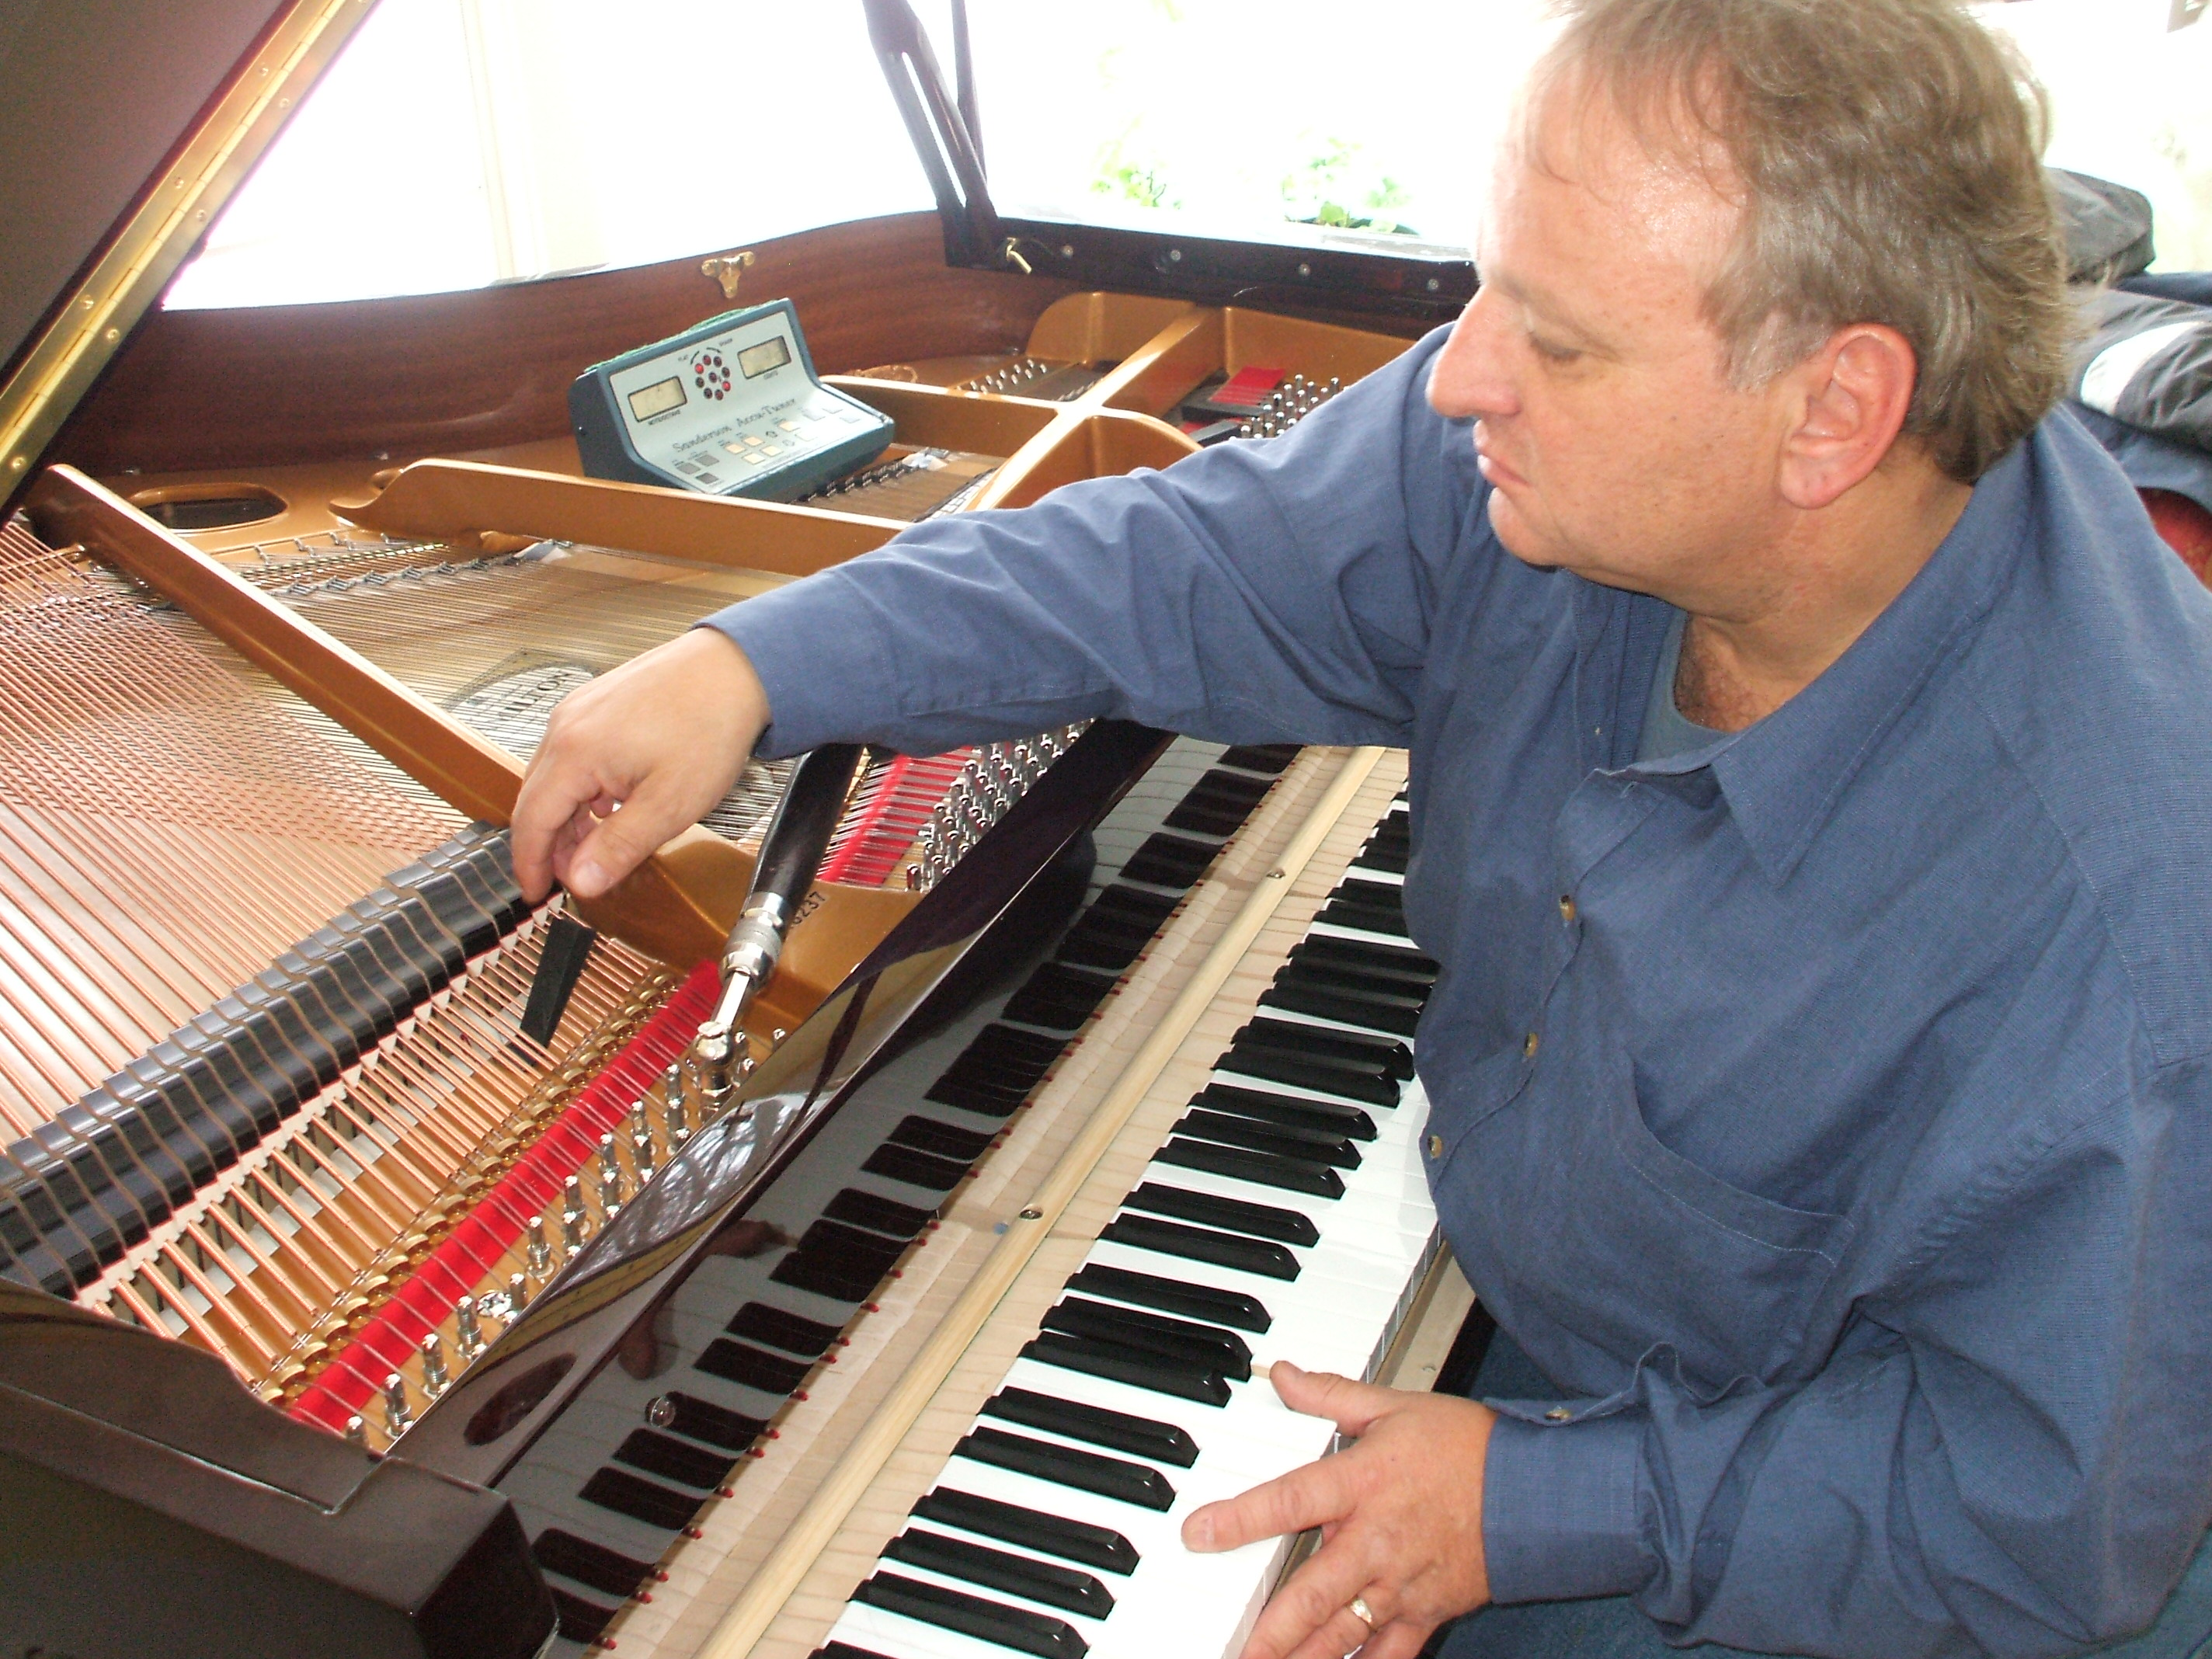
\includegraphics[width=0.75\textwidth]{images/tuner}
		\caption[Afinador de pianos]{\label{fig:tuner} Afinador de pianos. \cite{tuner}}
	\end{figure}
	
	De acuerdo a esto, la afinación cromática de cada nota sigue una sucesión 
	geométrica, referida a la frecuencia natural de vibración de cada nota:
	
	\begin{equation}
		f_i = f_{i-1} * 2^{\frac{1}{12}} = f_{i-1} * \sqrt[12]{2}
	\end{equation}
	
	El proceso de afinación consiste en que el técnico afinador, valiéndose de 
	un \textbf{diapasón}, afina las tres cuerdas que corresponden al $La_3$ y, 
	a partir de ahí, se basa en la \textbf{serie armónica} para afinar el resto 
	de notas.
	
	La frecuencia a la que una cuerda vibra depende de su masa, de su longitud 
	y de su tensión: \cite{cuerda}
	
	\begin{equation}
		f = \frac{\sqrt{\frac{T}{\mu}}}{2L}
	\end{equation}
	
	\begin{description}
		\item[$f$] Frecuencia de vibración.
		\item[$T$] Tensión que soporta la cuerda.
		\item[$L$] Longitud de la parte vibrante de la cuerda.
		\item[$\mu$] Densidad lineal de la cuerda ($\frac{m}{L}$).
	\end{description}
	
	% Bibliografía -------------------------------------------------------------
	
	\clearpage
	\addcontentsline{toc}{section}{Referencias}
	\bibliographystyle{acm}
	\nocite{piano}
	\bibliography{piano}
\end{document}

